\begin{figure}[!t]
\centering
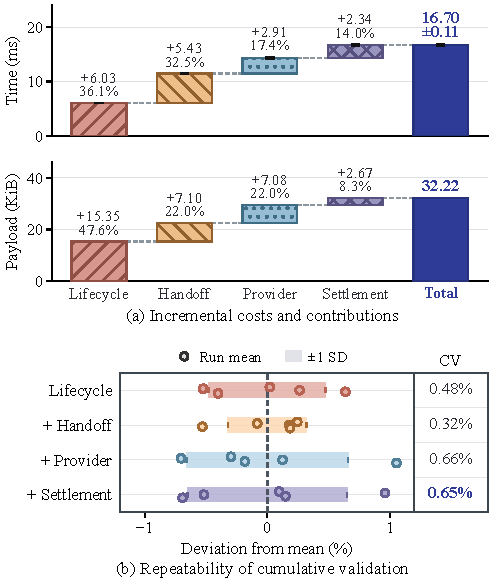
\includegraphics[width=\columnwidth]{f_component_waterfalls.pdf}
\caption{Costs and repeatability on prebuilt eight-call, 32-event fixtures.
(a) Waterfalls show mean paired increments in validation time and selected
payload; labels give increments and shares of the final total. Time whiskers
show sample SDs of cumulative configuration means. Totals include the
0.47\,$\mu$s/22\,B baseline. (b) Points show the signed percentage deviation
of each run mean from its cumulative configuration mean; shaded intervals
span $\pm1$ sample SD, with CV reported at right. Five historical runs each use
1,000 measurements after 100 warmups per configuration. Serialization is
outside the validation timer.}
\label{fig:f-component-costs}
\end{figure}
